% TikZ code for K_4^(3) using predefined edge colors
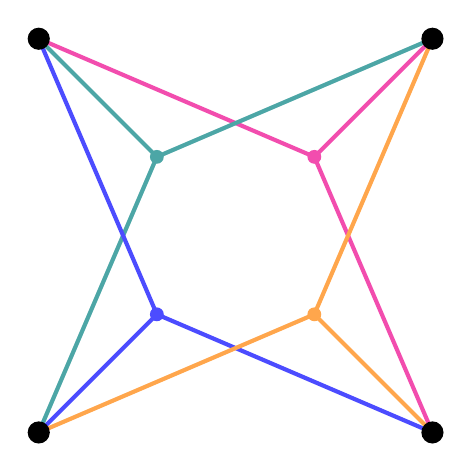
\begin{tikzpicture}[scale=1]
\coordinate (V1) at (0, 5);
\coordinate (V2) at (5, 5);
\coordinate (V3) at (5, 0);
\coordinate (V4) at (0, 0);
\coordinate (R0) at (3.500, 3.500);
\draw[line width=1.5pt, color=magenta!70!white] (R0) -- (V1);
\draw[line width=1.5pt, color=magenta!70!white] (R0) -- (V2);
\draw[line width=1.5pt, color=magenta!70!white] (R0) -- (V3);
\fill[color=magenta!70!white] (R0) circle (2.5pt);
\coordinate (R1) at (1.500, 3.500);
\draw[line width=1.5pt, color=teal!70!white] (R1) -- (V1);
\draw[line width=1.5pt, color=teal!70!white] (R1) -- (V2);
\draw[line width=1.5pt, color=teal!70!white] (R1) -- (V4);
\fill[color=teal!70!white] (R1) circle (2.5pt);
\coordinate (R2) at (1.500, 1.500);
\draw[line width=1.5pt, color=blue!70!white] (R2) -- (V1);
\draw[line width=1.5pt, color=blue!70!white] (R2) -- (V3);
\draw[line width=1.5pt, color=blue!70!white] (R2) -- (V4);
\fill[color=blue!70!white] (R2) circle (2.5pt);
\coordinate (R3) at (3.500, 1.500);
\draw[line width=1.5pt, color=orange!70!white] (R3) -- (V2);
\draw[line width=1.5pt, color=orange!70!white] (R3) -- (V3);
\draw[line width=1.5pt, color=orange!70!white] (R3) -- (V4);
\fill[color=orange!70!white] (R3) circle (2.5pt);
\fill[black] (V1) circle (4.0pt);
\fill[black] (V2) circle (4.0pt);
\fill[black] (V3) circle (4.0pt);
\fill[black] (V4) circle (4.0pt);
\end{tikzpicture}